% my main entry on the LaTeX report for my master thesis

\documentclass[a4paper]{report}
\usepackage[acronym,toc]{glossaries}
\usepackage{url}
\usepackage{graphicx}
\usepackage{float}

\makeglossaries

%my glossary (for the TM LHC tune)

\newglossaryentry{bunch}{
   name=bunch,
   description={
      particules trapped inside an \gls{RF} bucket circulating in the 
      machine},
   plural=bunches}
\newglossaryentry{bucket}{
   name={bucket},
   description={
      at every \gls{RF} period in the \gls{rffreq} there is a 
      bucket, in each of these bucket a particles bunch can potentially be 
      stored in the ring},
   plural={buckets}}
\newglossaryentry{rffreq}{
   name={RF frequency ($f_{\textsc{rf}} = 400{\rm MHz}$)},
   description={
      the base frequency of the \gls{RF} in the \glspl{cavity}; in the case of
      the LHC this frequency is 400.789MHz. This frequency dictates the number of
      buckets that the machine can have}}
\newglossaryentry{cavity}{
   name={cavity},
   description={
      \gls{RF} structure made to accelerate the particles; it uses a high power 
      radio frequency into a resonating structure to increase the energy 
      of the particles and provide longitudinal focusing},
   plural={cavities}}
\newglossaryentry{VME}{
   name={VMEbus},
   description={
      a computer bus standard widespread at CERN, in the case of the LHC
      \gls{RF} the bus has a larger board and some of the pins are used to 
      route custom signals between cards}}
\newglossaryentry{kicker}{
   name={kicker},
   description={
      device in an accelerator that can kick the beam transversally, used to
      kick the beam in or out (injection or extraction kicker) of the beam pipe 
      but also in our case excite the beam transversally},
   plural={kickers}}
\newglossaryentry{damper}{
   name={transverse damper},
   description={
      device in an accelerator that damp the transverse oscillation of the 
      beam by applying a transverse electric field},
   plural={dampers}}
\newglossaryentry{tune}{
   name={betatron tune},
   description={
      the betatron tune is the frequency of the oscillations of the 
      \glspl{bunch} divided by the revolution frequency ($f_0$)}}
\newglossaryentry{h}{
   name={harmonic number ($H$)},
   description={
      the harmonic number is the number of bucket an accelerator can have in 
      the ring, in the case of the \gls{LHC} 35'640}}
\newglossaryentry{FFTW}{
   name={FFTW},
   description={
      is a C subroutine library for computing the discrete Fourier transform 
      (DFT) in one or more dimensions, of arbitrary input size, and of both 
      real and complex data (as well as of even odd data, i.e. the discrete 
      cosine sine transforms or DCT/DST)}}
\newglossaryentry{OpenCV}{
   name={OpenCV},
   description={
      Open Source Computer Vision is a library in C/C++ under BSD license that
      has a lot of image manipulation and computer vision algorithms in highly
      optimized version.
   }
}

% my acronym list

\newacronym{ADT}{ADT}{Accelerating \Gls{damper} Transverse}
\newacronym{MKQA}{MKQA}{tune \gls{kicker}}
\newacronym{BBQ}{BBQ}{diode-based base-band-tune}
\newacronym{LHC}{LHC}{Large Hadron Collider}
\newacronym{DSP}{DSP}{Digital Signal Processor}
\newacronym{FPGA}{FPGA}{Field-Programmable Gate Array}
\newacronym{FFT}{FFT}{Fast Fourier Transform}
\newacronym{DFT}{DFT}{Discrete Fourier Transform}
\newacronym{GPU}{GPU}{Graphic Processing Unit}
\newacronym{GPGPU}{GPGPU}{General Purpose Graphic Processing Unit}
\newacronym{CPU}{CPU}{Central Processing Unit}
\newacronym{BPM}{BPM}{Beam Position Monitor}
\newacronym{RF}{RF}{Radio Frequency}
\newacronym{BI}{BI}{Beam Instrumentation}
\newacronym{CO}{CO}{Control group}
\newacronym{OP}{OP}{Operation}
\newacronym{CERN}{CERN}{European organization for nuclear research}
\newacronym{Hepia}{Hepia}{Haute {\'e}cole du paysage, d'ing{\'e}nieurie et d'architecture de Gen{\`e}ve}
\newacronym{MD}{MD}{Machine Development}
\newacronym{SVD}{SVD}{Singular Value Decomposition}
\newacronym{OpenCL}{OpenCL}{Open Computing Language}
\newacronym{OpenGL}{OpenGL}{Open Graphic Language}
\newacronym{API}{API}{Application Programing Interface}
\newacronym{SLC}{SLC}{Scientific Linux CERN}
\newacronym{CUDA}{CUDA}{Compute Unified Device Architecture}
\newacronym{HLSL}{HLSL}{High Level Shader Language}
\newacronym{GLSL}{GLSL}{OpenGL Shader Language}
\newacronym{CMW}{CMW}{Controls Middle-Ware}
\newacronym{CCC}{CCC}{CERN Control Center}
\newacronym{MIT}{MIT}{Massachusetts Institute of Technology}
\newacronym{flops}{flops}{floating-point operations per second}
\newacronym{FESA}{FESA}{Front-End Software Architecture}
\newacronym{SFP}{SFP}{Small form-factor pluggable transceiver}
\newacronym{NFS}{NFS}{Network File System}
\newacronym{ADTDSPU}{ADTDSPU}{ADT VME DSP card getting the values from the pickups}
\newacronym{CVS}{CVS}{Concurrent Versions System}
\newacronym{GPL}{GPL}{GNU Public License}
\newacronym{GSL}{GSL}{GNU Scientific Library}
\newacronym{SR4}{SR4}{the ADT surface building, location of the Faraday cage}


\title{Betatron tune measurement in the LHC damper using GPU}
\author{Fr\'ed\'eric Dubouchet}
\date{\today}

\begin{document}

\maketitle

\begin{abstract}
This paper describes the betatron tune measurement in the \gls{LHC} at the
\gls{CERN} including the present hardware and the future possible 
implementations using the \gls{ADT} acquisitions. The \gls{ADT} data have to 
be processed to be able to extract the \gls{tune}. This paper studies the use
of \glspl{GPU} to process \gls{bunch} position acquisition data.
\end{abstract}

\tableofcontents
\listoffigures
\listoftables

% Introduction
%
%	Motivation
%	State of the Research
%	Goals and Outline

\chapter{Introduction}

\section{State of knowledge}

In a particle accelerator, the charged particles circulate around the ring and oscillate due to the magnets and the accelerating structures. The accelerating structures, in the \gls{LHC} supra-conducting \glspl{cavity} apply a strong electrical field that oscillates at the \gls{rffreq} to particles in order to collect and accelerate particles in \glspl{bunch} inside a frequency \gls{bucket}.

The particles inside a bucket are oscillating longitudinally along the ring and transversally in the vertical and horizontal plane. The longitudinal oscillations are damped by the beam control system. But the transversal oscillations must be damped by a separate system~: the \gls{ADT}\cite{Benews11,Zhabitsky:1141925}.

One of the key parameters of the accelerator is the betatron tune. The betatron tune, $Q$, is the quotient of the betatron oscillation and the particle frequencies.

$$f_\beta = Q * f_0$$

This value allow us to check if the particle beam is stable and don't reach any dangerous instabilities.

% Literacy survey
\section{Tune measurement in the LHC}

In order to measure the betatron tune in an accelerator we use \glspl{BPM}. These monitors are able to measure the position of the beam in the vacuum chamber.

In the present setup \gls{BI} group is using their \gls{BBQ} \cite{Boccardi:1156349} system to acquire the tune over a certain number of machine turn (256 to 128'000). This can work as a passive instrument or as an on demand system by exciting 12 \glspl{bunch} in the beam with the \gls{MKQA}. \Gls{ADT} has also been used for tune measurement excitation\cite{HofleEvian10}. 

In normal operation, as the \gls{ADT} is active, it is difficult to have a good picture of the excited bunches and make a fine tune measurement~: the oscillations created by the \gls{MKQA} are damped by the \gls{ADT}. There have been studies to disable the \gls{ADT} for a certain number of bunches in order to get a better tune measurement\cite{HofleEvian11}, but this may not be sufficient.

% The source of Ideas
\section{Proposed system}

The \gls{ADT} also have \glspl{BPM} and these can have per bunch measurement\cite{BphMeas07}. This could allow a much precise measurement. But due to the high among of data to be processed (estimated to 640 mega bytes per seconds for each \gls{BPM}) dedicated hardware is needed to compute the correct tune\cite{HofleChamonix12}.

In order to be able to apply direct correction to beam oscilliation the \gls{tune} has to be measured at a high frequency, this has been estimated by \gls{BI} to be between 5 and 10[Hz], once every 100 to 200[ms].

During the 2012 normal operation of the \gls{LHC}, data has be acquired using the \gls{ADT} acquisition system and data processing techniques has been tried to asses the modification that will be needed in order to make a reliable \gls{tune} measurement at a reasonable rate\cite{HofleChamonix12}.

The current \gls{VME} implementation has some serious issues in particular the bus is quite slow the data rate of the bus is around 40 megabits per seconds. The data need to either be processed on the acquisition board or to be off-loaded to another computer using the serial link available on the board\cite{Baudrenghien:1124094}.

\subsection{DSP on VME board}

\Glspl{DSP} are able to compute \glspl{FFT} at high rate and these are used already in the machine at different places to make high speed feedback loops. The question is~: is it fast enough to compute all the \glspl{FFT} needed, \glspl{DSP} are two orders of magnitude slower than \glspl{GPU}. We also would have to develop a completely new system in order to be able to use them, in fact we don't have \glspl{DSP} in the present \gls{ADT}. The cost of development and the complexity of the deployment should also be studied.

\subsection{FPGA pre-processing on VME board}

Like in the approach using \glspl{DSP} on VME boards, the question of computing power is still unsolved. We already have in house experience and we already have a lot of \gls{FPGA} installed in the \gls{ADT}. But if we want to do it we will have to create a new card able to replace the existing one and to make the computation. This mean create a potential problem in the existing setup. The cost is also to be studied we have to develop a new card, test it and install it in the \gls{LHC}. Also the number of card and FPGA is not well understood, it could be anywhere between 4 and 3000. 

The biggest issue for FPGA computing been the fact that you need something like ~100M bytes of memory to store the temporary values for computation of only one beam plane.

\begin{quotation}
96'265'920 Bytes from 2024 points times 2 for complex times 2880 the number of bunches times 4 size of float times 2 because you need to double buffer.
\end{quotation}

This is far too much memory to be access simultaneously by a single \gls{FPGA}. In case we want to make these computations on \gls{FPGA} it would cost a lot of money in hardware and development.

\subsection{GPU off-board computing}

This solution can be integrated easily in the present setup. The present acquisition cards already have a digital output and could be used to transfer the data in another crate that could do the computations. The \glspl{GPU} are cheap (compare to the price of developing a new \gls{VME} card) and easily scalable. The \gls{GPU} should have largely enough computing power to be able to make the \glspl{FFT}. Another interesting aspect of this solution is the ability to test it using \gls{CPU}.

\section{Problem definition}

Show how to implement a GPU based system that can deliver a tune value for each beam and planes at a frequency that allow the system to be responsive enougth to allow tune correction to be applied automatically. 

   \subsection{Algorithm}

   We need the tune frequency and we have the tune position per bunch, we have to calculate the FFT to move from time to frequency domain. Then we need to identify the tune in the transformation.

   \subsection{Hardware}

   \begin{figure}[H]
	\caption{ADT acquisition hardware}
	\centering
	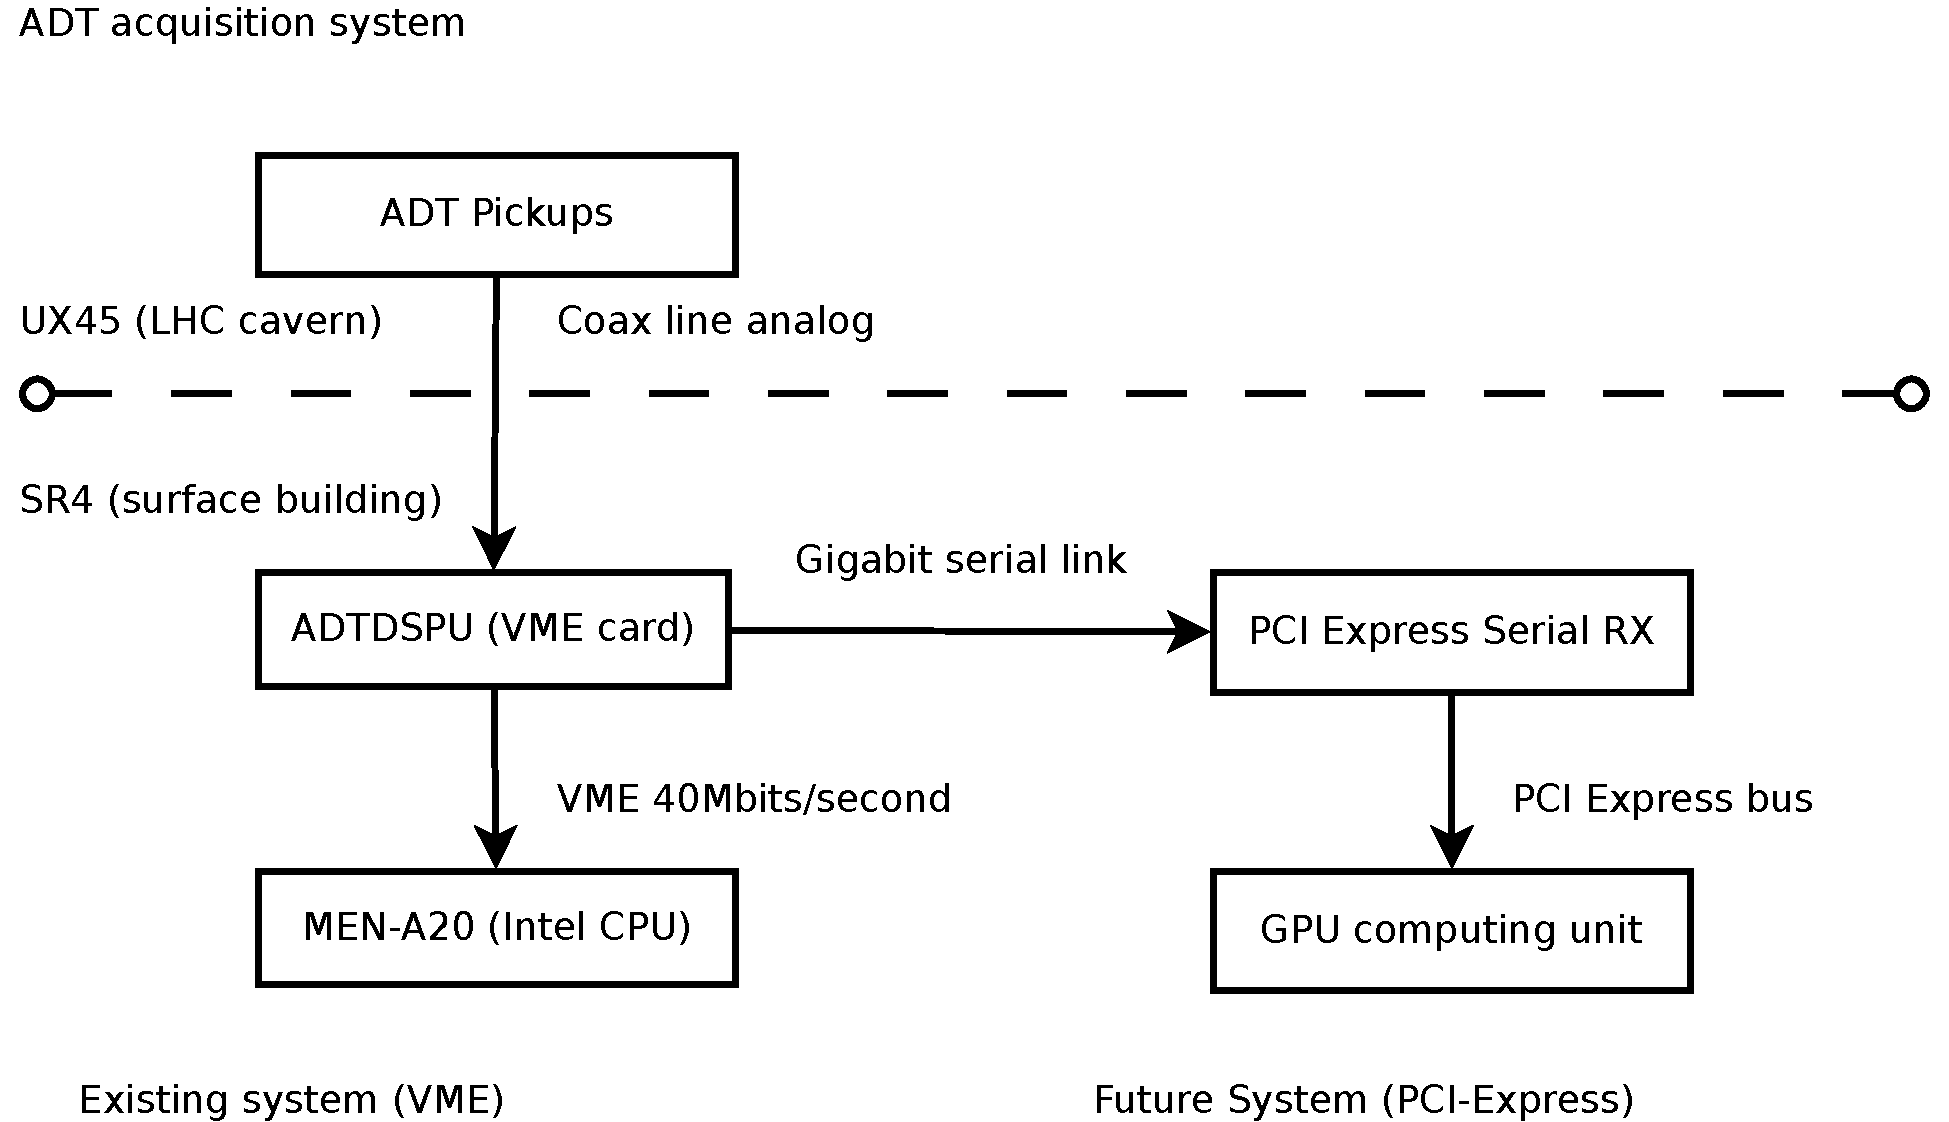
\includegraphics[scale=0.3]{acquisition.pdf}
	\end{figure}

   Per bunch position mesearment has to be avalable to the system for each beam and each plane. This should be provided from the ADTDSPU card and has to be transfered through a serial link to the CPU/GPU crate for computation.

   We need a card in the CPU/GPU crate to unserialize the data and transfer them to the GPU memory. It may be possible to copy from the acquisition card directly to the GPU memory.

   And finally fast enougth GPU to process the data. The number and the type of card should be looked at. The possibilty for expantion should be kept as the possibility to implement other algorithms.
   
   \subsection{Timing}

   Acording to \gls{BI} we have to provide the tune measurement betweeen 5 Hz and 10 Hz. This mean that the transfer and the computation has to be made in less than 200 ms.

   At a higher frequency because of the acquisition frequency (11 kHz) the precision may be unsufficient (Nyquist–Shannon sampling theorem).
% Results
%
%	some important things to know
% 	experimental parts in the chapter results
%	numerical results or so-called data
%	order of presentation
% 	cross references

\chapter{Results}

During the \glspl{MD} we were able to acquire some data from the \gls{LHC} \gls{ADT} system. We used off-line analysis on these data to try the different algorithm and assess the feasibility of the project.

\section{Notch filter}
\label{sec:notch}

A notch filter is used to cut the low frequencies amplifying the frequencies around the tune by a factor around 2 and then diminish the tail like for the low frequencies (the frequency domain being anyway symmetric due to the fact that we are converting real values. It will not be used in the final as we are only interested in the band between 0.25 to 0.35. For every sample the filter takes the present sample and subtract the next element. 

$$y_{[n]} = x_{[n]} - x_{[n + 1]}$$

As visible on formula one value is dropped at the end of the data set but as we are using radix 2 \glspl{FFT} the data is cut to a power of 2.

This is a differential filter and as we are only interested into the frequencies around the tune this has no incidence on our results and allows for a better visualization of the spectrograms.

\section{FFT}
\label{sec:FFT}

The Fourier transform is a mathematical operation that moves a function from a temporal domain to a frequency domain using an integral relation. In our case, we are treating sampled signals for which the integrals reduce to a summation, the transform being referred to as the \gls{DFT}. The specific term ``\gls{FFT}'' refers to a fast algorithm to compute the \gls{DFT} when for example the number of samples $N$ equals is power of 2.

\subsection{Definition}

The \gls{DFT} is a discrete transform. It transforms a series of complex numbers into another series, the \gls{DFT} of the original series.

$$ x_0,...,x_{N -1} \in \mathbb{C} $$

$$ X_{k} = \displaystyle\sum\limits_{n = 0}^{N -1} x_{n}e^{-i 2 \pi k \frac{n}{N}} $$

In order to compute the \gls{DFT} one must compute $N$ values $N$ times. The complexity is of order $N$ times $N$~: $ \mathcal{O}(N^{2}) $.

The most commonly used \gls{FFT} algorithms are based on a divide-and-conquer approach similar to the algorithm of Cooley and Turkey~\cite{Cooley65}. The computation of a \gls{DFT} of length N is done by splitting the input sequence into a fixed small number of subsequences, compute their \gls{DFT}, and assemble the outputs to build the final sequence. If the split and assembly are linear in time the complexity becomes~:

$$ \mathcal{O}(N \log_{2}(N)) $$

In the present case the parallelization is happening on the first N of the complexity so the complexity is divided by the number of core (up to to half of $N$ in radix 2 version). 

This is further reduced (in our case) by the fact that we calculate a number of \glspl{FFT} together equal to the number of bunches.

\subsection{FFTW}

\Gls{FFTW} is an implementation of the \gls{DFT} that adapts the algorithm to the hardware in order to maximize the performances~\cite{fftw05}. It is widely regarded as one of the fastest implementation of an \gls{FFT} on a \gls{CPU}.

It was selected as a reference for our implementation. As \gls{OpenCL} can be run directly on a \gls{CPU}, it is possible to compare the time performances between the \gls{OpenCL} code running on \gls{CPU} and the \gls{FFTW} version (see section~\ref{sec:perf}).

It is under GPL license and can be purchased from the \gls{MIT} for commercial purposes. It is used in many commercial and scientific package and software. For example, it is used by MATLAB~\cite{matlab_fftw}.

\subsection{FFT with OpenCL on GPU}

The \gls{FFT} version used in the software is derived from Eric Bainville's version. This is the reference implementation of \gls{FFT} on \gls{OpenCL} and is now the version distributed by Apple\cite{bainville11}. For the sake of simplicity restrict ourself to the radix~2 version of the implementation.

On \gls{GPU} the \gls{OpenCL} result is the same than the one using \gls{FFTW} with the advantage to be faster on recent \gls{GPU}. The kernel is called a number of times equal to the size of the vector and then 11 times in the case of 2048 points ($\log_{2}{2^{11}} = 11$). A second dimension is used to pass the multiple vector.

\subsection{FFT with OpenCL on a CPU}

As \gls{OpenCL} is also able to run on a \gls{CPU} we used the same code than the one used on a \gls{GPU} on a \gls{CPU} yielding same results. It is interesting to note that the time is very similar to the implementation using \gls{FFTW}.

\section{Amplitude}
\label{sec:amplitude}

The amplitude is the length of the complex vector composing the \gls{FFT}; it is equal to the euclidean norm. 

$$\mid x + i y \mid \equiv +\sqrt{x^2 + y^2}$$ 

There are different ways to compute the norm of a 2-dimensional vector in \gls{OpenCL} and all of them seem to work equally well in our test.

\section{SVD}
\label{sec:SVD}

It was suggested by Rama Calaga to use \gls{SVD} in order to diminish the noise and improve the visibility of the tune in the frequency domain. The idea is to take the raw data and use the multiple bunches as a second dimension of the matrix $M$ using SVD, $M$ containing turn by turn data. One can suppress the values in the singular value matrix ($\Sigma$) that are off a certain scale, recompose the $M'$ matrix with less noise.

$$M = U \Sigma V^{T}$$ 

This was first tested in the framework of this work on generated data by Wolfgang H{\"o}f\/le~\cite{HofleEvian10}. Unfortunately we have only 6 bunches in our dataset per acquisition so it is not possible to make this work with the present set up. The $\Sigma$ matrix will only be 6 by 6 and it is not easy to suppress values with a noticeable impact on the signal to noise ratio.

Taking more than one acquisition can at least give some idea on the speed of processing and feasibility. The SVD was implemented using the GNU Scientific Library (with double precision float for the SVD). Speed efficiency is difficult to estimate as we can see on table~\ref{tab:SVD} for the same number of sample, 100 in this table, we have a big variation of speed if we try to use different acquisitions.

\begin{table}[H]
\caption{SVD speed correlation with acquisitions bunches for a 100 by 2048 $M$ matrix}
\label{tab:SVD}
\centering
\begin{tabular}{|l|l|l|}
\hline
Bunches & Acquisitions & Time \\
\hline
5 & 20 & 0.15 s \\
4 & 25 & 0.30 s \\
2 & 50 & 2.04 s \\
1 & 100 & 16.9 s \\
\hline
\end{tabular}
\end{table}

So it is very difficult to estimate the time the computation would take with the real data. We have to keep in mind that these computation where done using double precision as single would probably be enough, these computation were also done using a single thread (SVD is quite difficult to parallelize) and only done on \gls{CPU}.

There is a way to make these computation on \gls{GPU}\cite{Lahabar09} and the estimation is that is would be around 5 times better than on a \gls{CPU}.

\section{Performances}
\label{sec:perf}

Computations were made with an accumulation to simulate the number of bunches that could be present in the final version (2880). As 6 bunches were acquired we used 500 successive acquisitions to make, close to the maximum of 2880.

Different strategies were used to try to improve the performance as shown in Figure~\ref{fig:PCFlow}. Pipelining was also used (not used on the Figure as it is difficult to estimate time when using pipelining) and tested on different type of hardware.

The hardware used was mainly the Tesla M2090 based on a Fermi chip. This chips has more cores than a CPU and we can see an improvement with respect to computing speed as shown in Table~\ref{tab:speed}. Table~\ref{tab:fermi} shows the characteristics of the Tesla Fermi card family.

\begin{table}[H]
\caption{NVIDIA Fermi hardware available on the market}
\floatfoot{Source : NVIDIA\cite{nvidia}}
\label{tab:fermi}
\centering
\begin{tabular}{|l|l|l|}
\hline
Features & Tesla M2090 & Tesla M2075 \\
\hline
\hline
Peak double performance & 665 Gflops  & 512 Gflops \\
\hline
Peak single performance & 1331 Gflops & 1030 Gflops \\
\hline
Memory bandwidth (ECC off) & 177 GB/sec & 150 GB/sec \\
\hline
Memory size (GDDR5) & 6 GB & 6 GB \\
\hline
CUDA cores & 512 & 448 \\
\hline
\end{tabular}
\end{table}

However, if we have a look on the different cards that are available today on the market we see that the new generation should provide even better result and are available today. These cards show around 5 times the number of \gls{CUDA} core and around 10 times the number of \gls{flops} as shown in Table~\ref{tab:kepler}.

\begin{table}[H]
\centering
\caption{NVIDIA Kepler hardware available on the market}
\floatfoot{Source : NVIDIA\cite{nvidia}}
\label{tab:kepler}
\begin{tabular}{|l|l|l|l|}
\hline
Features & Tesla K20X & Tesla K20 & Tesla K10 \\
\hline
\hline
Peak double performance & 1.31 Tflops & 1.17 Tflops & 190 Gflops \\
\hline
Peak single performance & 3.95 Tflops & 3.52 Tflops & 4577 Gflops \\
\hline
Memory bandwidth (ECC off) & 250 GB/sec & 208 GB/sec & 320 GB/sec \\
\hline
Memory size (GDDR5) & 6 GB & 5 GB & 8GB \\
\hline
CUDA cores & 2688 & 2496 & 3072 \\
\hline
\end{tabular}
\end{table}


\subsection{Pipelining}

To improve the performances one of the options is to remove all waiting time between the different operations on the \gls{GPU}, as shown in Figure~\ref{fig:PCFlow}. The different operations done on the \gls{GPU} that are done sequentially can be pipelined.

Pipelining mean that one will not wait for all the sub-operations to be finished for a certain task on a data set, but will already start treating the next set. The first operation is copying the memory from the \gls{CPU} to the \gls{GPU} which takes a certain time. As soon as some of the data is copied the computing could start.

In \gls{OpenCL} the different commands are queued and this command queue can be flushed (with the command endQueue). To make the pipelining work the only thing to do is to only flush at the end when all the computing has been queued. Of course some attention should be kept to avoid problems with modules writing or reading data that has not yet been read or written.

In our case this means that the copying of the data from the \gls{CPU} to the \gls{GPU} the preparation of the data, the \gls{FFT} itself, and the amplitude computation, the accumulation and getting back the values to the \gls{CPU} are queued together in one go.

That allows us to have a 3 to 10\% improvement on the performances, but it is difficult then to estimate the computing time of individual steps consequently the values shown in Figure~\ref{fig:PCFlow} are without pipelining.

\subsection{Memory}

Copying memory from and to the \gls{GPU} can be expensive time wise, as shown in Figure~\ref{fig:PCFlow}. Copying 3000 times 2048 values in short (2 bytes) takes around 10 ms. This is the reason why it is important to make the accumulation on the \gls{GPU} and avoid the \gls{FFT} computation of 3000 times 2048 complex values in float (8 bytes). It would have cost at least 40 ms to copy these values back to the \gls{CPU}. 

The 20 ms shown in Figure~\ref{fig:PCFlow} correspond to half the values because we can cut half of the result as the \gls{FFT} computed it in real only so the result is mirrored.

\subsection{Time}

\begin{table}[H]
\caption{Speed for 3000 acquisitions of 2048 points}
\centering
\label{tab:speed}
\begin{tabular}{|l|lrrcr|}
\hline
Device & Type & Threads & Speed [GHz] & Pipeline & Time [ms] \\
\hline
\hline
Xeon X5650 & FFTW & 12 & 2.67 & N/A & 291 \\
Xeon X5650 & OpenCL & 12 & 2.67 & enable & 284 \\
Xeon X5650 & OpenCL & 12 & 2.67 & disable & 288 \\
\hline
i7-3720QM & FFTW & 8 & 2.6 & N/A & 310 \\
i7-3720QM & OpenCL & 8 & 2.6 & enable & 272 \\
i7-3720QM & OpenCL & 8 & 2.6 & disable & 273 \\
\hline
\hline
Tesla M2090 & OpenCL & 512 & 1.3 & enable & 35 \\
Tesla M2090 & OpenCL & 512 & 1.3 & disable & 37 \\
\hline
GeForce 650M & OpenCL & 384 & 0.9 & enable & 355 \\
GeForce 650M & OpenCL & 384 & 0.9 & disable & 365 \\
\hline
\end{tabular}
\end{table}

Time performances were computed using the timing library from boost \cite{boost} on different hardware, \glspl{GPU} and \glspl{CPU}, with and without pipeline enable as shown on table \ref{tab:speed}.

The time performances between \gls{FFTW} and \gls{OpenCL} on a \gls{CPU} are very close, hence the radix 2 implementation on \gls{GPU} should be solid.

On a dedicated \gls{GPU} like the Tesla M2090  the performances are around 10 times better than on a modern \gls{CPU}. This is very encouraging and means that on the latest generation hardware we should be able to achieve even better performances.

\section{Spectrogram}
\label{sec:spectrogram}

A Spectrogram is a time-varying spectral representation of a signal. The signal is transformed via \gls{FFT} from time domain to spectral domain. Each transformation produces a line in this case and is tagged with the time of the acquisition. the amplitude is used to have a single representation of both real and imaginary part of the result.

As we do a normalization per acquisition on the spectrum at the end of the computing we have a representation of the highest value with highest color (white). If the amplitude is weaker we have a darker representation of the color (black). To have a finer grain in representation intermediate color was chosen in this case blue as you can see in figure \ref{fig:squeeze} \ref{fig:ramp} and \ref{fig:adt_off}.

\begin{figure}[H]
\caption{Spectrogram with ADT off on the 16 October 2012 on vertical beam 1 during squeeze and collision}
\label{fig:squeeze}
\centering
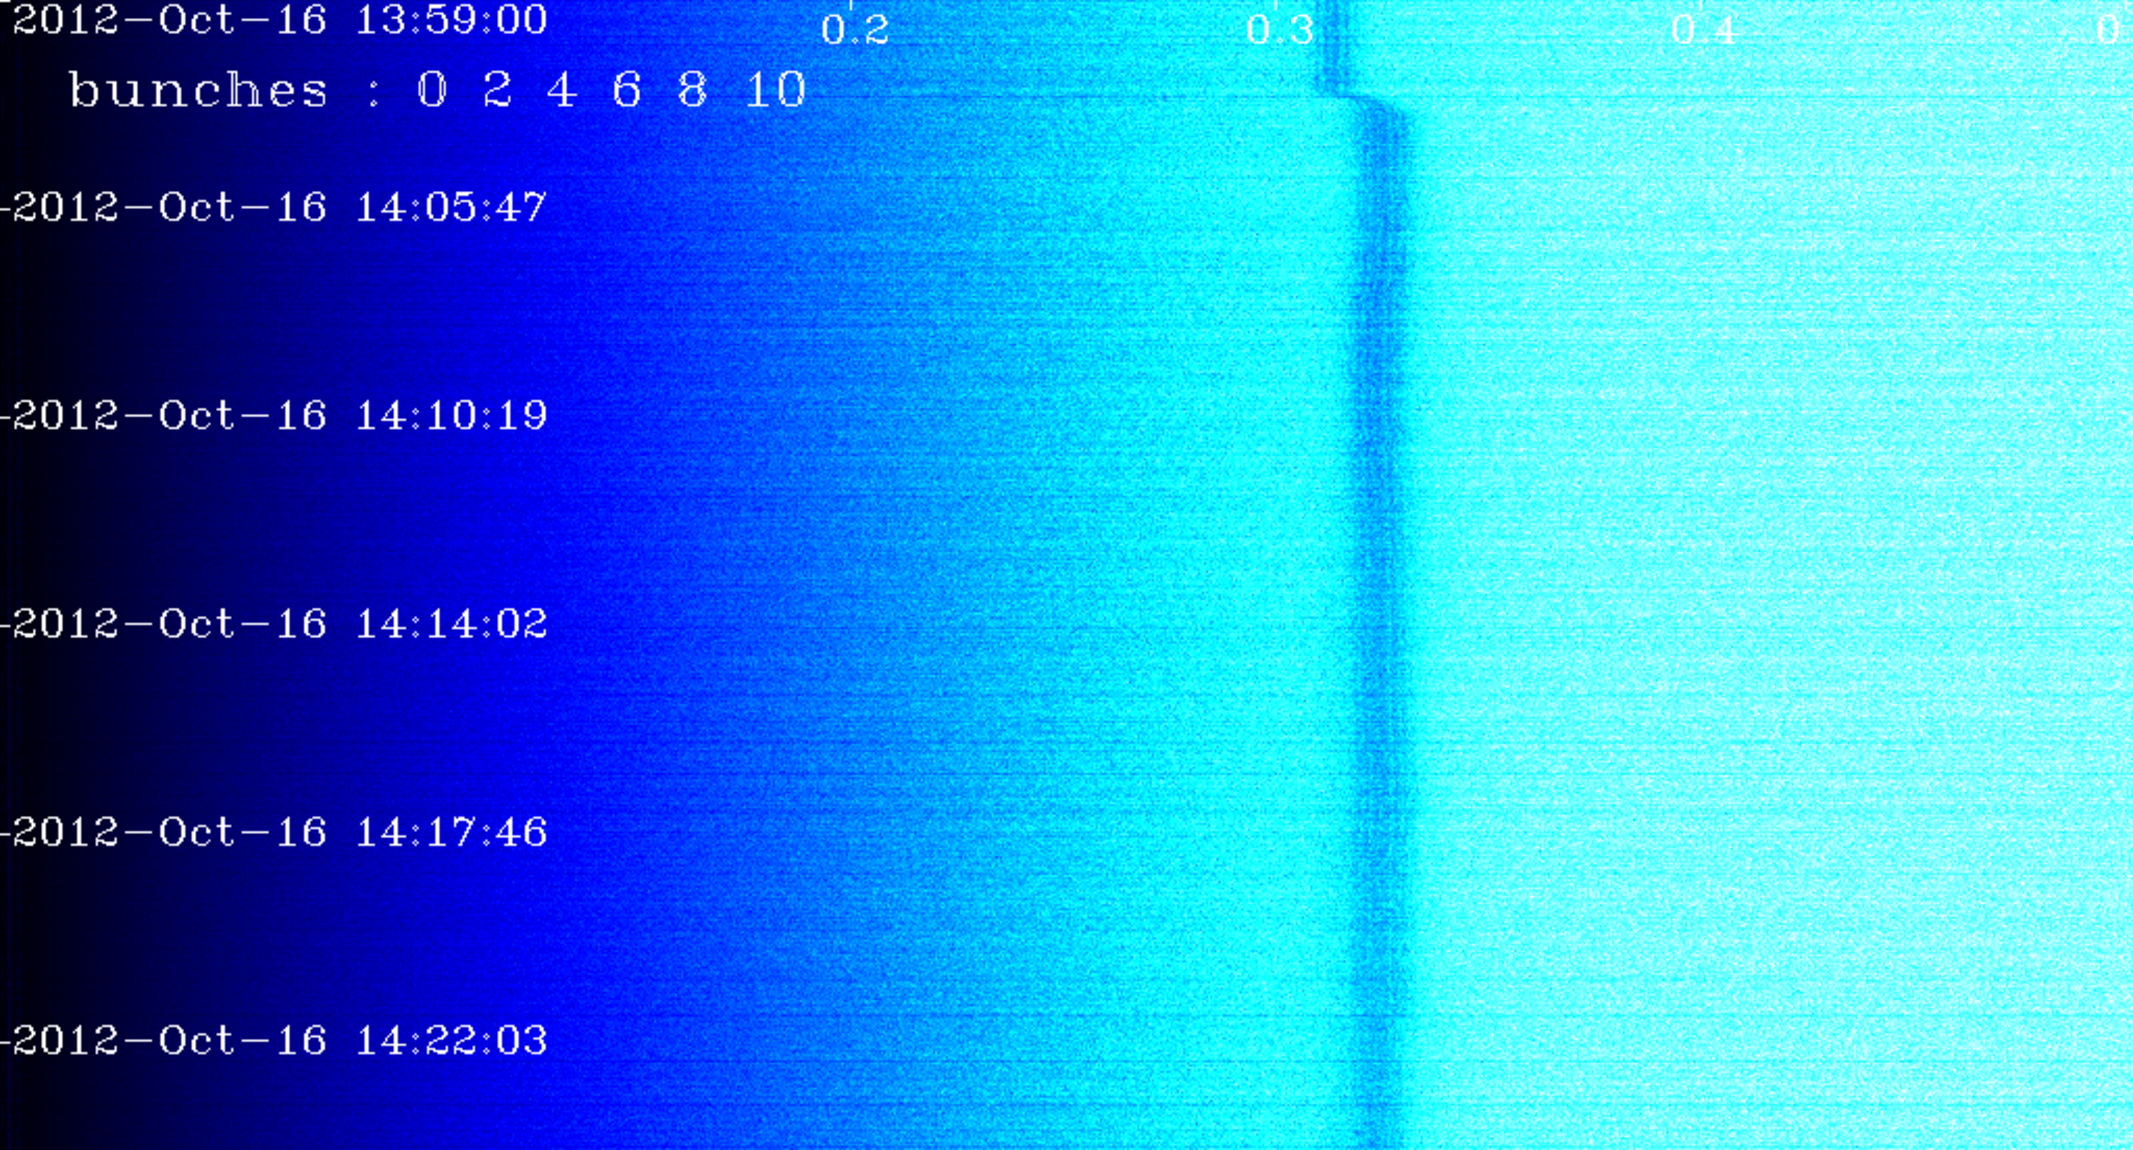
\includegraphics[scale=0.3]{md-121016-vb1-m1-6bunches-10acc-1359-1425-collision.pdf}
\end{figure}

The Spectrogram allow us to clearly see a mark in the signal that correspond to a region where the tune is suppose to be.
% Discussion

\chapter{Discussion}

Analysis of the spectrograms show a mark that can be high in intensity or be a trench in the signal. It is too early to assume this is the \gls{tune} but it is still very encouraging. It is possible to assess the feasibility of the tune measurement using \gls{GPU}.

\section{Observation}

During the three \glspl{MD} we acquired around 50 giga-bytes with both beam and both planes. This data was acquired in XML files and stored on the \gls{CERN} infrastructure. XML was chosen as it is easily accessible by both custom and commercial data analysis software.

Matlab was used as the first tool to check the data and try different algorithm but in the end the software was ready fast enough and flexible enough. Matlab ended to be only used for check and test purpose and all the analysis and discussion is based on the result obtain with the data analysis software (described in section~\ref{sec:data_analysis_software}).

\subsection{Without damper}

When the \gls{ADT} is off line there is a clear mark on the tune as shown in Figure~\ref{fig:adt_off}. There is still discussion on, it might be the tune or just a ripple of the tune. Some test could still be made, crosschecking with the \gls{BBQ}, changing the tune and looking in real time.

\begin{figure}[H]
\caption{Spectrogram with ADT off on the 16 October 2012 on vertical beam 1 before the ramp, 6 bunches 10 accumulations}
\label{fig:adt_off}
\centering
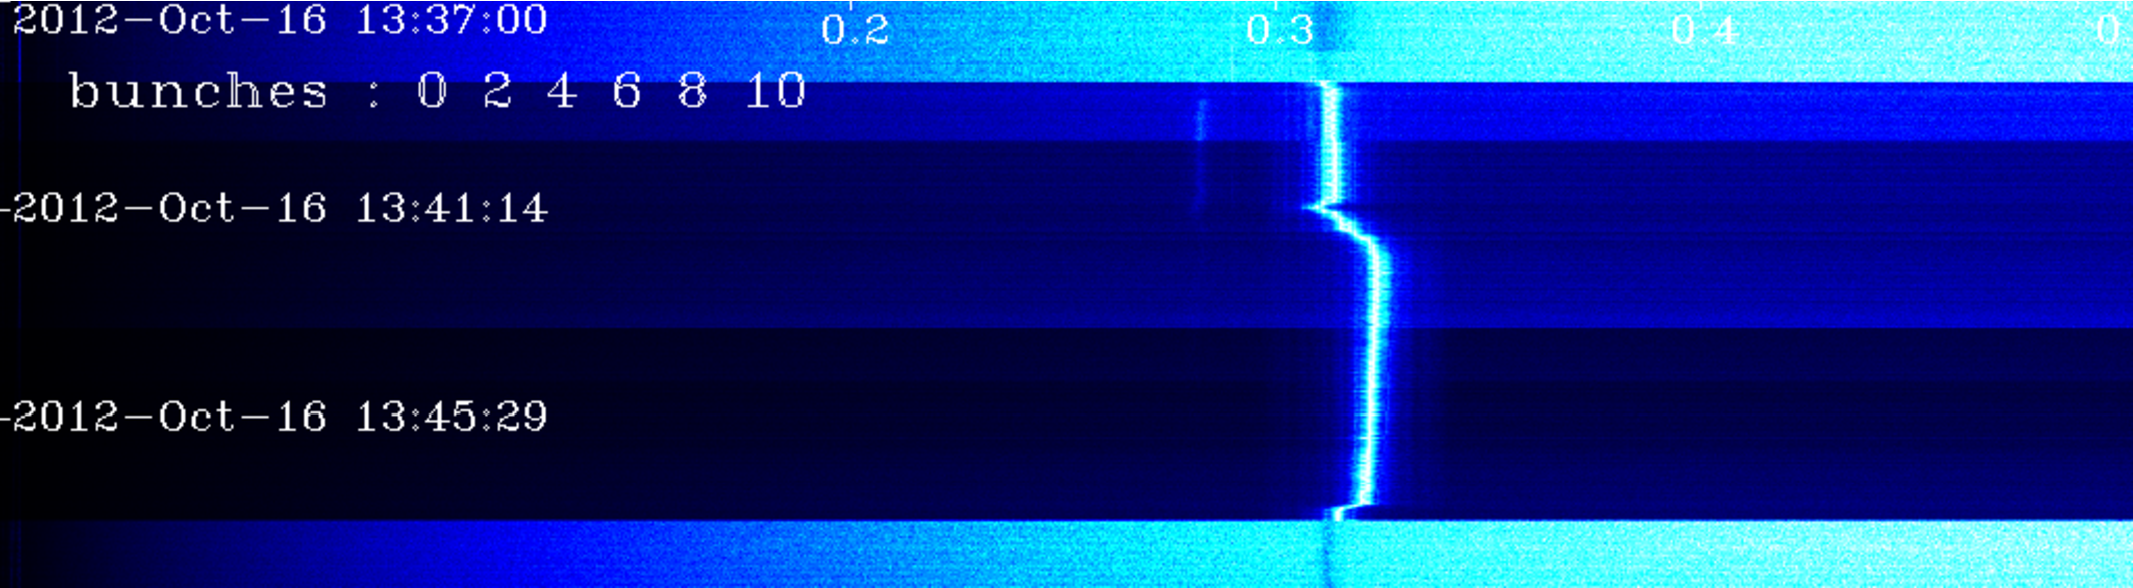
\includegraphics[scale=0.3]{md-121016-vb1-m1-6bunches-10acc-1337-1349-ADT-off.pdf}
\end{figure}

These observations are consistent with the gated-\gls{BBQ} result of 2012 \cite{Valuch12} and show that we can acquire the tune with the \gls{ADT} and get a clear bunch-by-bunch view of the tune even for only one bunch as shown in Figure~\ref{fig:bunch_0_adt_off}.

\begin{figure}[H]
\caption{Spectrogram with ADT off on the 16 October 2012 on horizontal beam 1 before the ramp, 1 bunch (0) 8 accumulations}
\label{fig:bunch_0_adt_off}
\centering
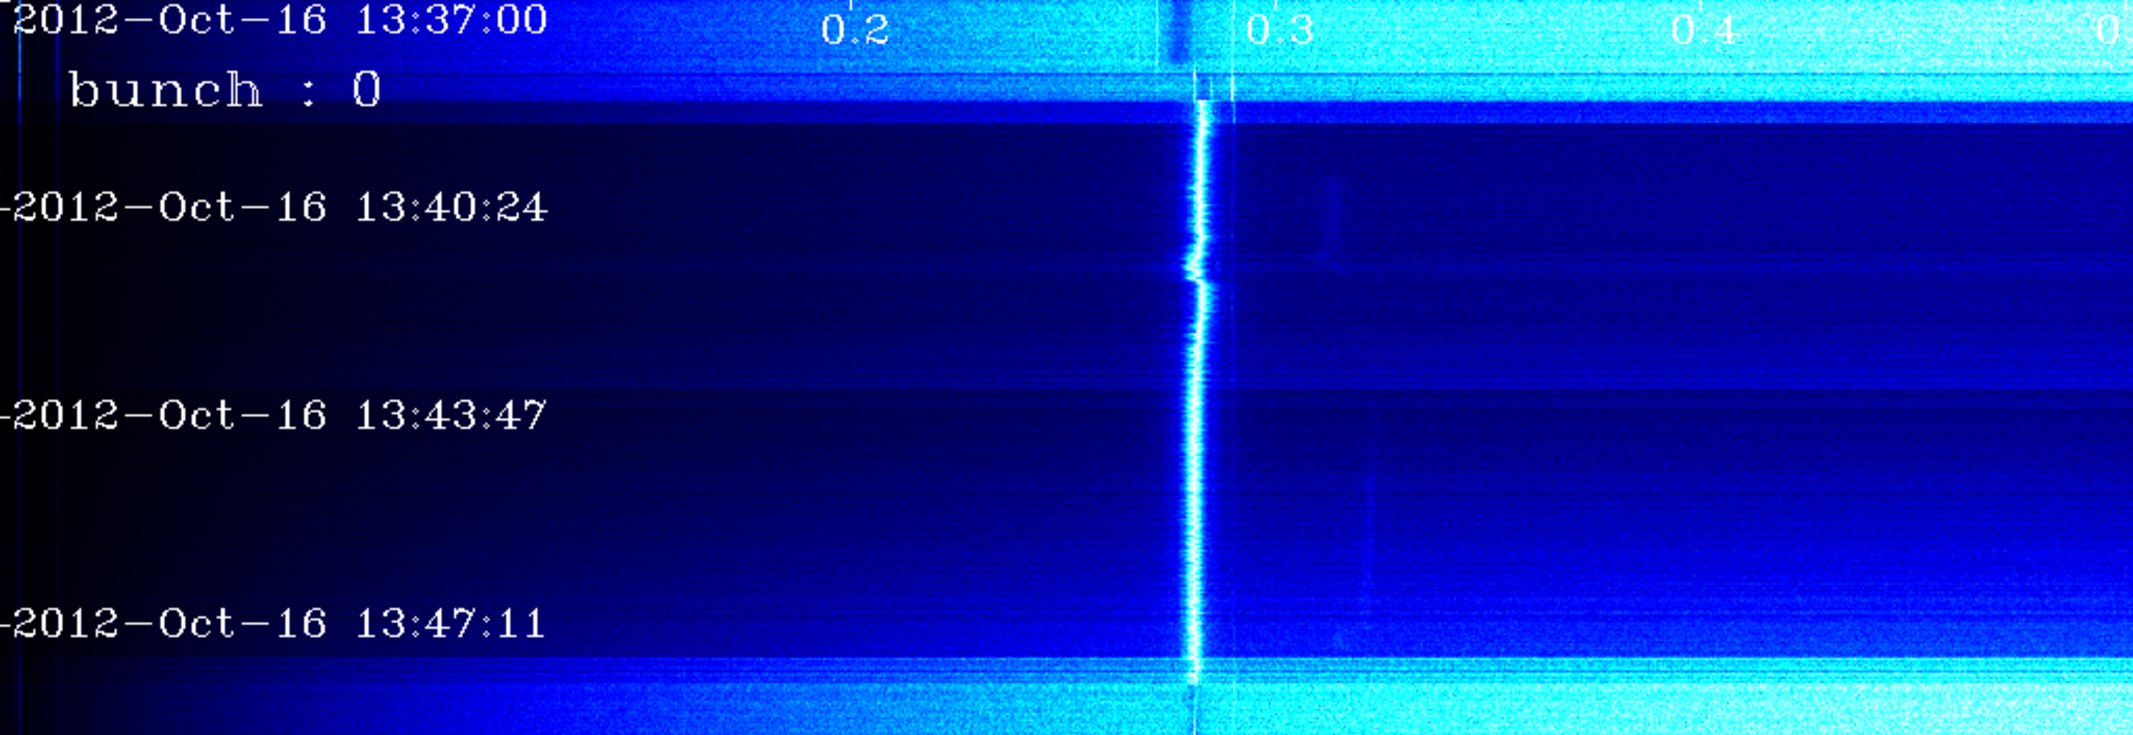
\includegraphics[scale=0.3]{md-121016-hb1-m1-bunch000001-8acc-1337-1349.pdf}
\end{figure}

\subsection{With damper}

When the \gls{ADT} is working the oscillations of the beam are damped by it, as a result the tune is less visible. But we should be able to see the effect of the tune on the damper if the damper is well adjusted to the beam. This mean that we should see a clear gap in the frequency around the tune frequency (or at the frequency at which the damper is operating, a frequency that should be close to the tune but not necessary be the tune itself).

This correspond to the spectrogram we see during operation as shown in
Figure~\ref{fig:ramp}. We also see in this figure the energy ramp
before collision. Before putting the beam in collision we do a squeeze
(operation during which we compress the beam size in the interaction
points, where the experiments are). The squeeze is changing the tune
and we can see it on the spectrogram around 14h03 on the figure
\ref{fig:ramp}.

\begin{figure}[H]
\caption{Spectrogram with damper working on the 16 October 2012 on vertical beam 1 during the ramp, 6 bunches 10 accumulations}
\centering
\label{fig:ramp}
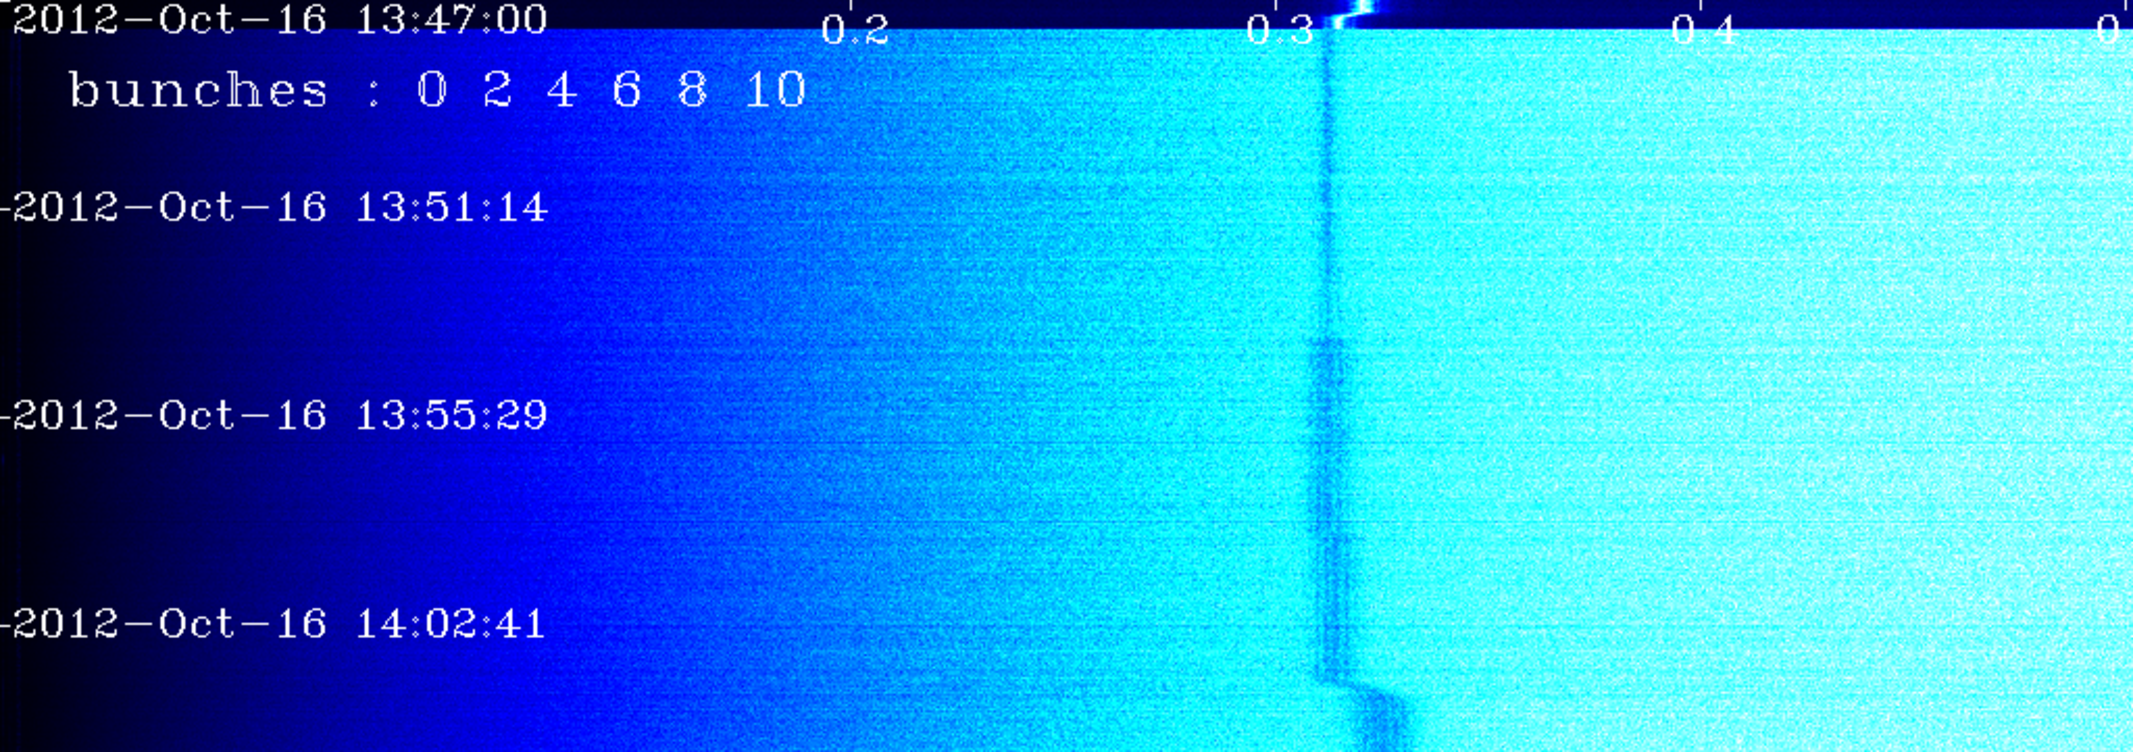
\includegraphics[scale=0.3]{md-121016-vb1-m1-6bunches-10acc-1347-1405-ramp.pdf}
\end{figure}

This could give us a good acquisition of the \gls{tune} during operation even when \gls{ADT} is on. This acquisition is made bunch-by-bunch. The question that is still up is how much is it sensible to the way the \gls{ADT} is set up. This has still to be tested in the machine by moving the tune while the \gls{ADT} is in operation and see if the acquisitions follows the tune.

\section{Data flow}

As the hardware is not present yet, the time and bandwidth of the whole system has to be estimated to see if it is doable in the constraint we have and that were exposed in the introduction. Estimation of the bandwidth and data flow is shown in Figure~\ref{fig:data_flow}.

\begin{figure}[H]
\caption{Acquisition data flow}
\label{fig:data_flow}
\centering
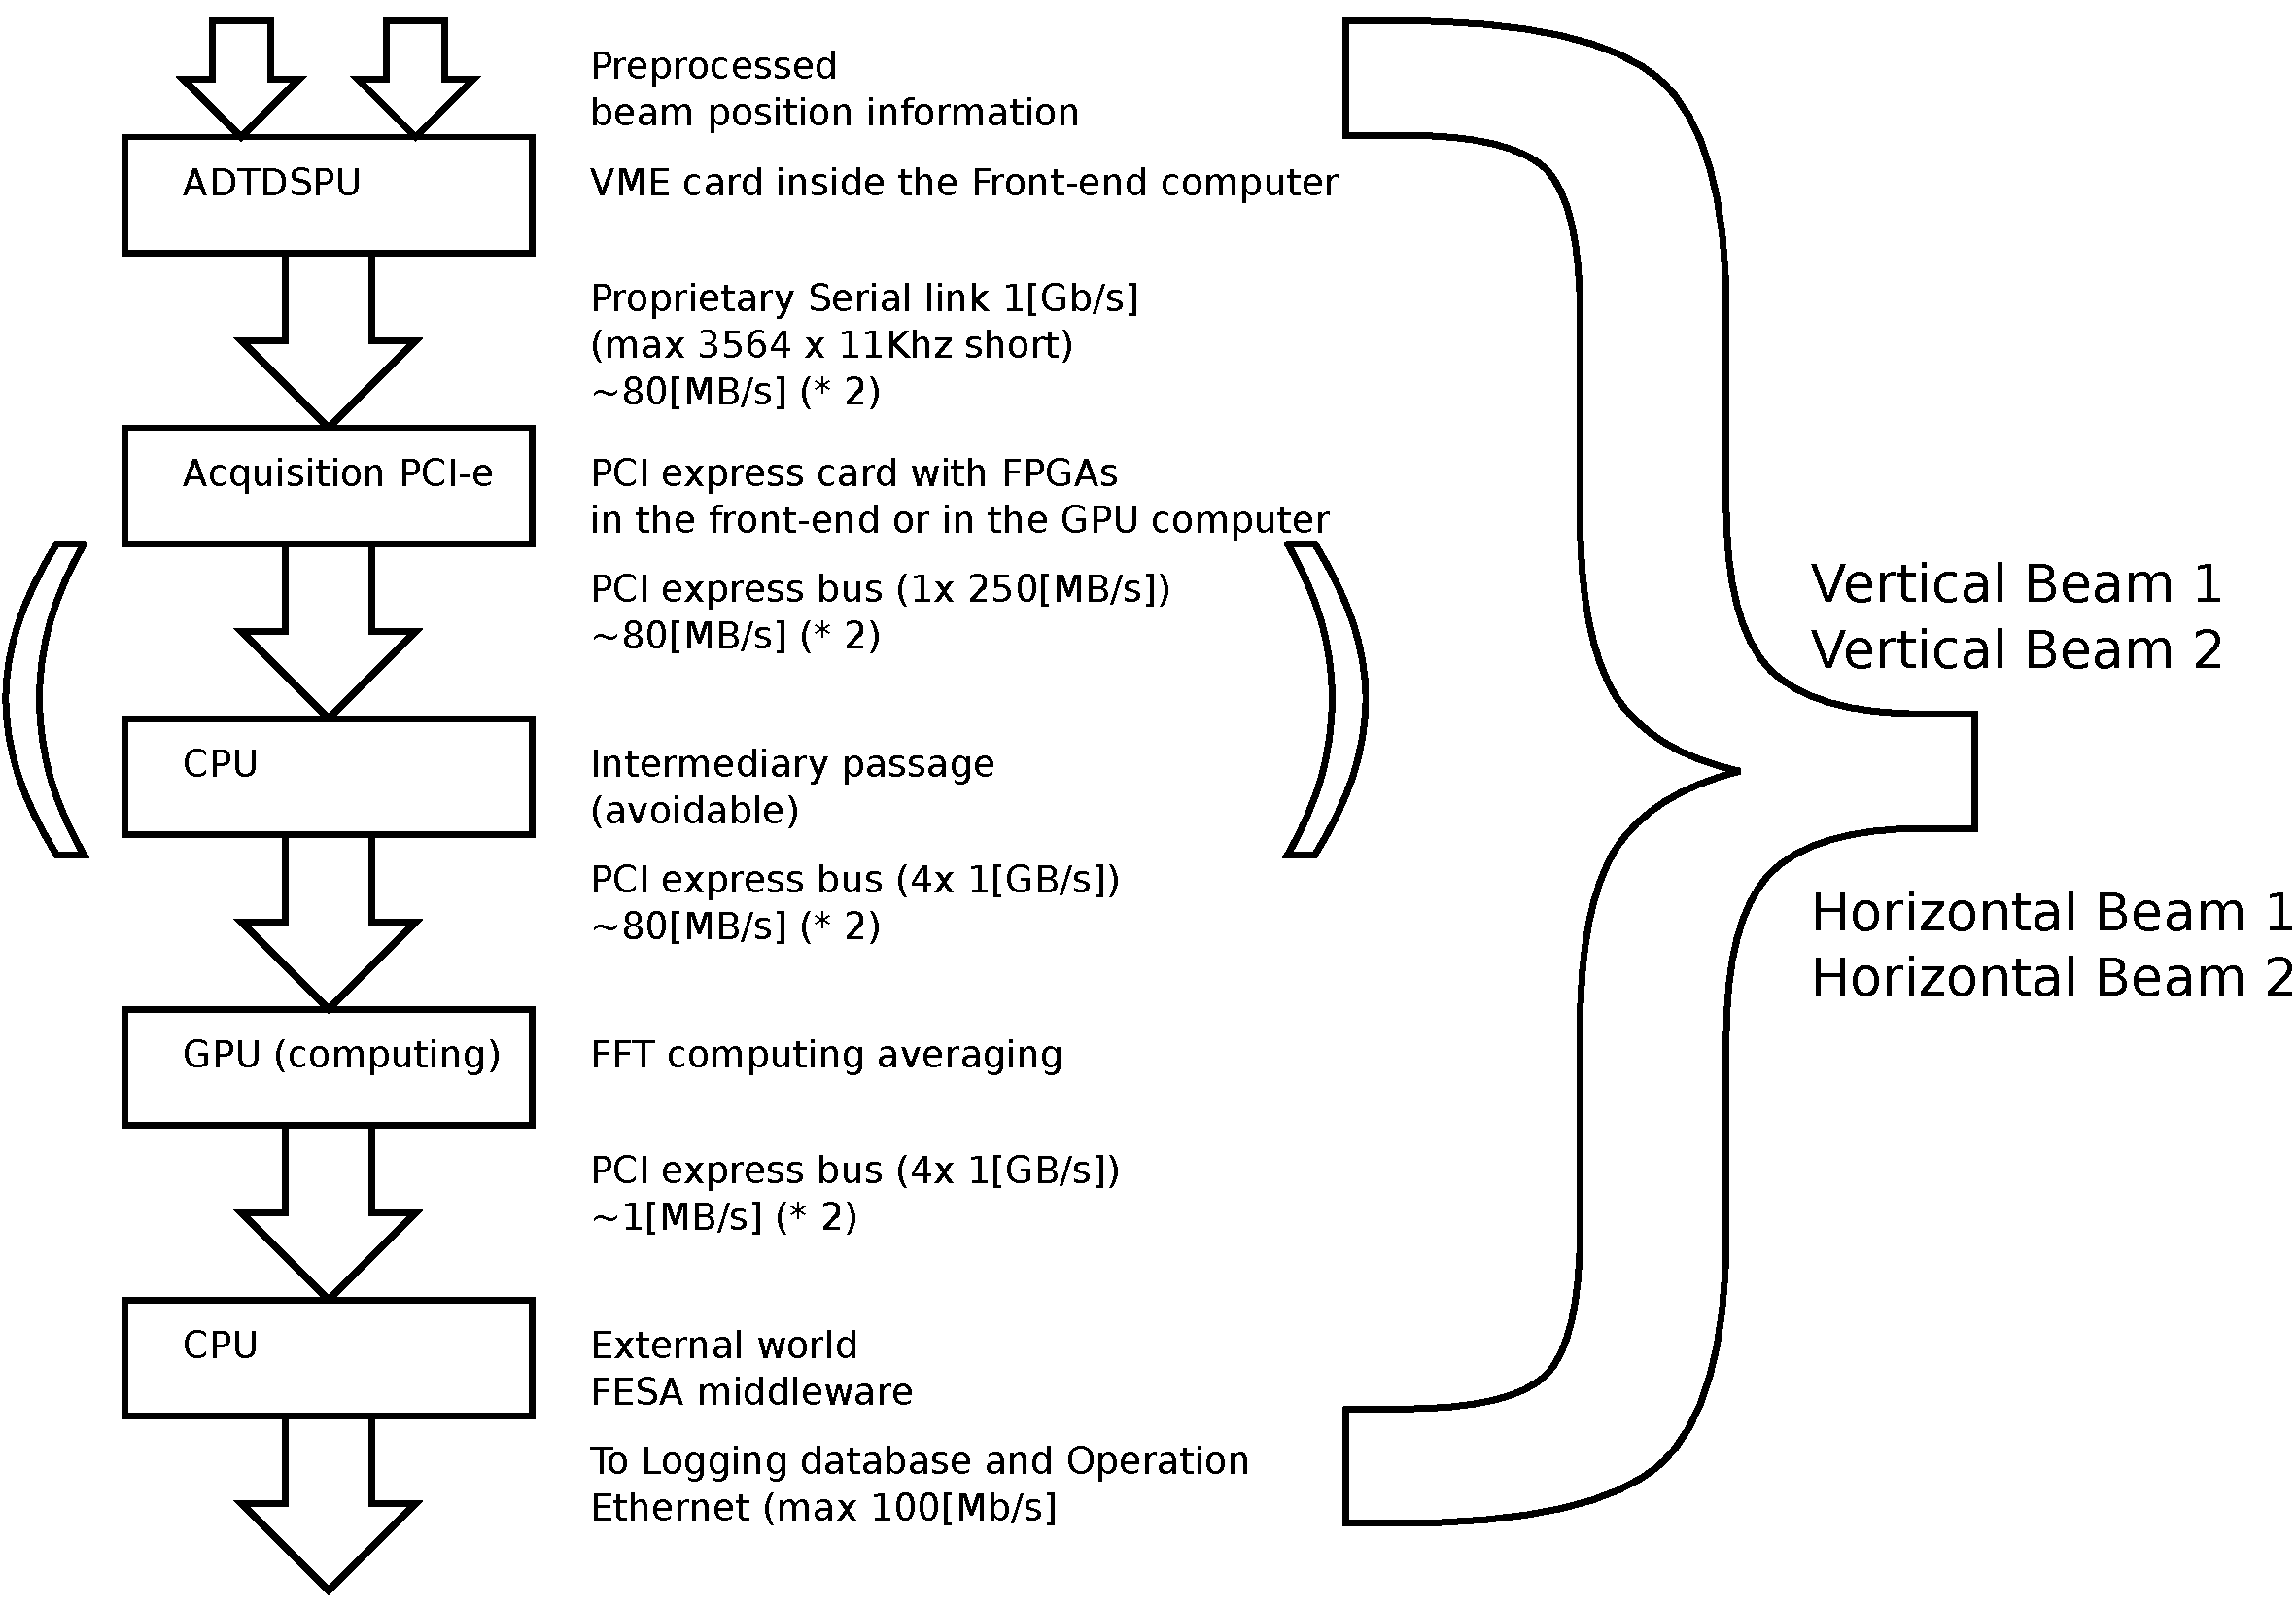
\includegraphics[scale=0.3]{dataflow.pdf}
\end{figure}

The data has to move from the acquisition card to the GPU by a series of steps, first from the card to the PCI crate (the one who contain the actual \glspl{GPU}). The problem being that the acquisition card is a \gls{VME} card and the VME bus is too slow to allow the full data to be streamed to the \gls{CPU}. 

We will use the giga-bit serial link already present on the VME
card. A receiver card will then receive the data in the PCI crate and
send it either directly to the \gls{GPU} memory or to the \gls{CPU}
and then to the \gls{GPU} memory.

The \gls{GPU} will make the computations necessary for the \gls{tune} measurement and will copy the results back to the \gls{CPU}.

As a final step we will use Ethernet to transmit the data back to the operation and eventually make the corrections needed.

\section{Hardware}

The present hardware does not allow us to acquire all the \glspl{bunch} of the machine and is in fact limited by constraints of the \gls{VME}. We have to upgrade various part of the hardware and to add the new computing device in order to be able to make on-line computation.

\subsection{ADT Acquisition boards}

The \gls{ADTDSPU} card will be redesigned and remade during the long shutdown 1 (\gls{LHC} upgrade from beginning of 2013 to 2015). It will be an upgrade of the whole card with \gls{tune} measurement and other needed features in mind.

\subsection{Serial link interface}

Serial link receiver has to be chosen and put into place in the new computing device to be able to receive the data and pass them to the \gls{GPU}. This card has to be fast enough to get the serial data from the serial link that comes from the ADTDSPU, have a PCI-express interface and \gls{SFP} interface on the front panel. 

It should also have a fast FPGA to de-serialize the bunch positions and send them to the PCI-express bus. To be able to communicate with the CPU, Linux drivers (with sources) have to be present.

A market survey revealed that commercial cards can fill up our needs.

\begin{figure}[H]
\caption{Nallatech PCIe-180}
\label{fig:nallatech}
\centering
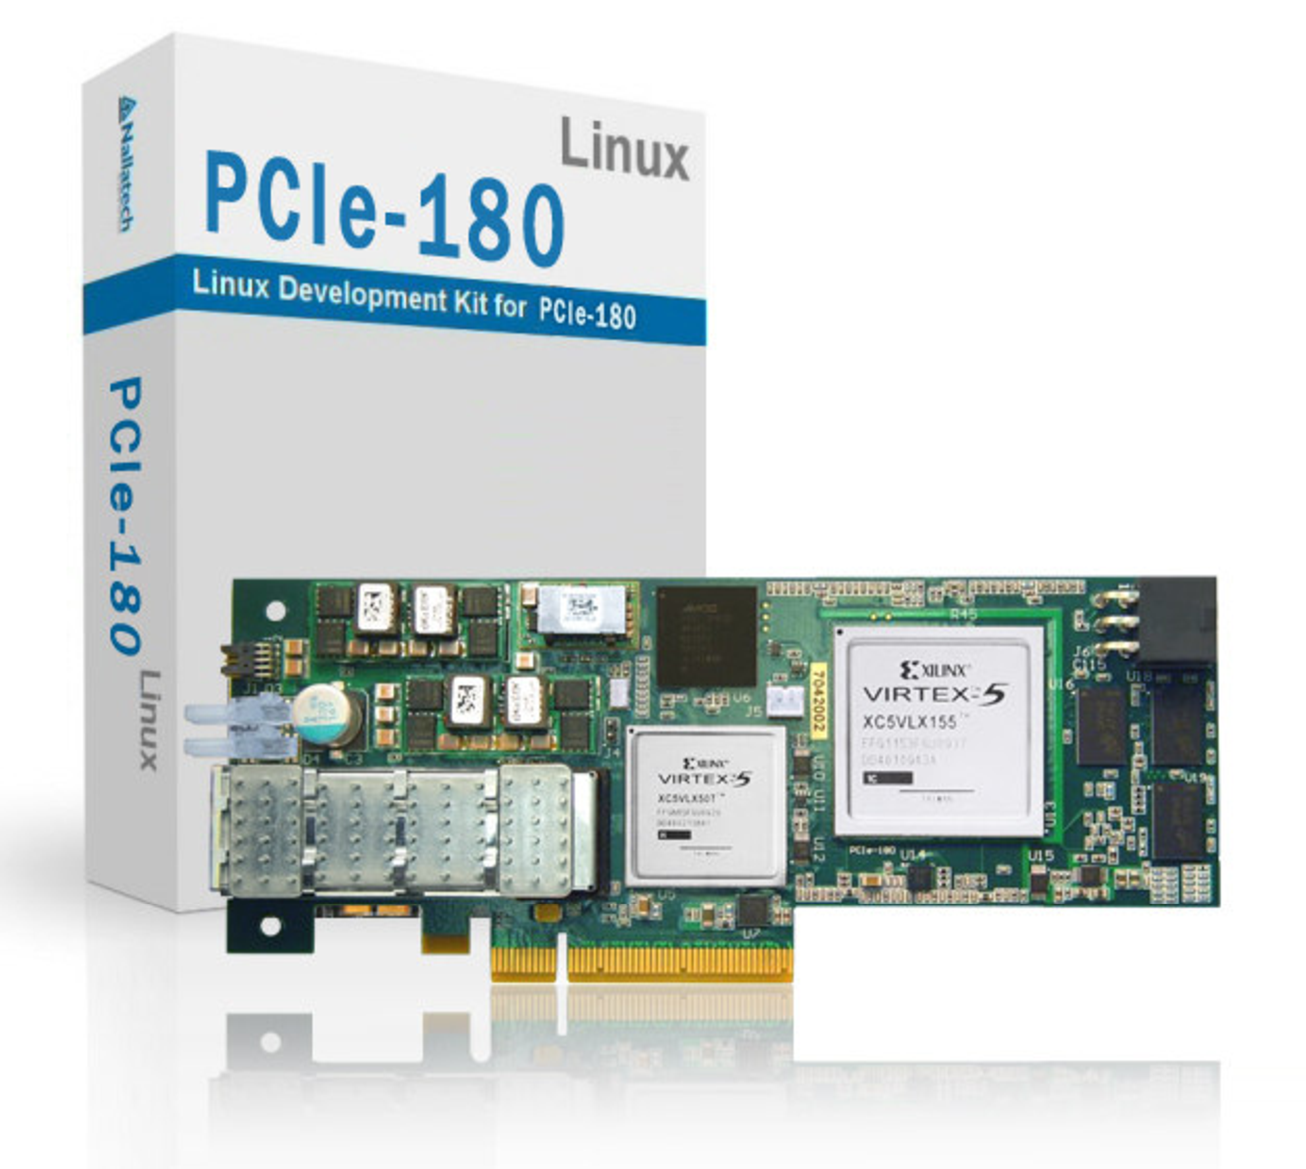
\includegraphics[scale=0.3]{Nallatech_PCIe-180.pdf}
\end{figure}

\gls{CERN} proposes a card that is made by \gls{CO} which could make a good match.

\begin{figure}[H]
\caption{CERN Simple FMC carrier (SPEC)}
\label{fig:spec}
\centering
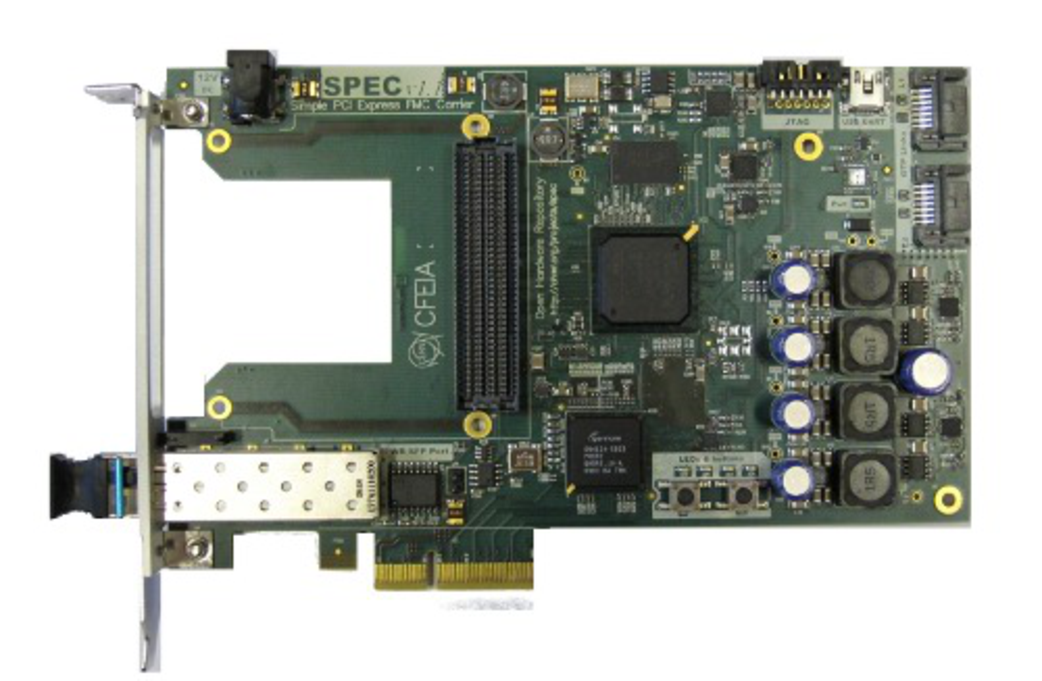
\includegraphics[scale=0.3]{spec_top.pdf}
\end{figure}

Table~\ref{tab:receiver_cards} show the different commercial and CERN solutions.

\begin{table}[H]
\caption{PCIe Giga bit link serial receiver card candidates}
\label{tab:receiver_cards}
\centering
\begin{tabular}{|ll|c|l|c|}
\hline
Name & Manufacturer & SFP & FPGA & Drivers \\
\hline
\hline
SPEC & CERN & 1 & Spartan-6 & yes \\
\hline
Virtex-5 LXT ML555 & Xilinx & 2 & Spartan-5 & no \\
\hline
Xilinx Virtex 6 & Hitech Global & 2 & Spartan-6 & no \\
\hline		
PCIe-287N & Nallatech & 4 & Kintex-7 * 2 & yes \\		
PCIe-180 & Nallatech & 2 & Virtex-5 & yes \\
\hline
\end{tabular}
\end{table}

For the moment the ``Nallatech PCIe-180'' seams to be the best match and we will probably order one to start testing with the present test setup.

\subsection{GPUs}

We need a computing device with at least 2 PCIe slots, one for the serial link receiver and one for the \gls{GPU} card. It should be a standardized crate with a powerful \gls{CPU} and possible expansion. Place has to be found in SR4, for either a for full crate or a smaller one.

We will probably start with a standard graphic card and then upgrade to a professional computing \gls{GPU} card (like NVIDIA Tesla series~\cite{nvidia}).

\section{Software}

Some software upgrade and redeployment is still necessary before the operational version is fully commissioned. New hardware will need new drivers and the software will have to be changed accordingly.

\subsection{Drivers}

The drivers for the \gls{ADT} acquisition card will need some update, changing the memory map and adjusting the drivers for the control registers. This should be quite straightforward.

A driver for the Serial link receiver card will be needed. If we use
one that is made inside \gls{CERN} we can have it made by the control
group (CO). In case we buy an off the shelf solution we will have to
make the driver ourself using the driver framework and the tools we
have.

\subsection{OpenCL}

The present \gls{OpenCL} code is able to compute the \gls{FFT} but we could try other algorithms in the future including hardware accelerated \gls{SVD}. This would ask some new \gls{OpenCL} development.

\subsection{Front-end}

Developing new software to control the new hardware are needed, the \gls{ADTDSPU} board is going to be changed and we are going to build a new computing front-end with a custom serial link receiver and a \gls{GPU}. New drivers and a software to stream data from the receiver card to the \gls{GPU} will be needed.

\section{Intermediate and Final setup}

A normal computer with a decent \gls{CPU} can be estimated to cost around 2'000 SFR and a top \gls{GPU} is around a 1'000 SFR. The reciever card should be in the same value band.

In case we have to move to rackable \gls{CPU} and a professional \gls{GPU} the price can go up to around 10'000 SFR per crate. This is still much cheaper than a \gls{VME} crate and custom cards.

\subsection{First prototype}

First prototype could be a normal computer with the receiver card and a graphic card \gls{GPU}. The idea is to test the hardware, and decide on the final setup.

This test will be made on the \gls{ADT} test setup in the laboratory and will be fed from the new version of the \gls{ADTDSPU} card.

\subsection{Final version}

At \gls{LHC} restart four crates will be deployed in \gls{SR4}. One for each ring and for each plane.

It will probably be build with industrial crate with a certain number of \gls{GPU} and a serial link receiver card. 

If the space allow it the test crate may be moved as well to be used on the test acquisition crate in \gls{SR4}.
% conclusion

\chapter{Conclusion}

\glsreset{GPU}
\glsreset{FFT}
\glsreset{LHC}

The betatron \gls{tune} is a critical parameter of a collider machine. In the \gls{LHC} the \gls{tune} acquisition is computed by doing \glspl{FFT} on an averaged value over all the bunches. In order to have a decent on-line \gls{FFT} computation of all individual bunches a faster method is needed. 

\Gls{GPU} used in graphic card are faster than normal \gls{CPU} for parallelized computations. Using \gls{GPU} we can accelerate \gls{FFT} computation by a factor of 10 especially if we have multiples \glspl{FFT} to be computed at the same time. This could, acording to the timing asked by the operation allow for a new on-line acquisition of the \gls{tune}.

New hardware will have to be deployed in the \gls{ADT} Faraday cage. This will in turn need new software to drive it. But is should be accessible as most of it is already present in the \gls{ADT} setup.

On-line computation of \glspl{FFT} for all the individual bunch is shown to be possible this will allow a better bunch-by-bunch surveillance of the beam and better statistic on what is causing transversal instabilities. This could allow to have a better tune acquisition and allow for a better beam time life in the \gls{LHC}.
% Methodology
%
%	Experimental Set-up
%	Model Equations

\chapter{Experimental}

\section{Estimation of the amount of data}

Presently the \gls{LHC} is working with an interval of 50ns between \glspl{bunch} this correspond to a bunch every 10 \glspl{bucket}. But the \gls{OP} is planning to move to 25ns \glspl{bunch} spacing this would mean 5 \glspl{bucket} between \glspl{bunch}. With the \gls{rffreq} we can compute the number of acquisitions per seconds.

$$for~50~ns~: \frac{400.789M}{20} = 20'039'450 \leq 2^{25}$$

$$for~25~ns~: \frac{400.789M}{10} = 40'078'900 \leq 2^{26}$$ 

This represent the amount of data for one pickup (\gls{BPM}), in the case of \gls{ADT} we have two of them per beam and per plane so as the \gls{LHC} has two rings and for each ring there are two transversal plane and there are two pickups per plane. This means we still have to multiply this value by eight.

$$for~50~ns~: 2^{25} * 8 = 2^{28}$$

$$for~25~ns~: 2^{26} * 8 = 2^{29}$$

As \glspl{FFT} on \glspl{GPU} start to be be faster than \glspl{CPU} around $2^{15}$ acquisitions it seems interesting to study this kind of system to compute the \gls{tune}.

\section{Measurement with the ADT}

In order to check the feasibility of the system and to have a good prototype the first test will be to excite some of the \glspl{bunch} and acquire the \gls{tune} using the \gls{ADT} during the end of 2012 run.

A piece of software has been developed that will acquire the bunch by bunch acquisition and compute various algorithm on the data using the \gls{CPU} and the \gls{FFTW} library in the \gls{CERN} infrastructure using \gls{CO} group control system and the \gls{OP} group infrastructure.

\section{Experimental Set-up}

   \subsection{Hardware}

	The experimental set up is not presently able to acquire more than a certain number of bunches due to memory limitation 16k and interupt frequency so during the \glspl{MD} only 6 bunches were acquired by bunch by planes.

\begin{figure}
\caption{ADT acquisition hardware}
\centering
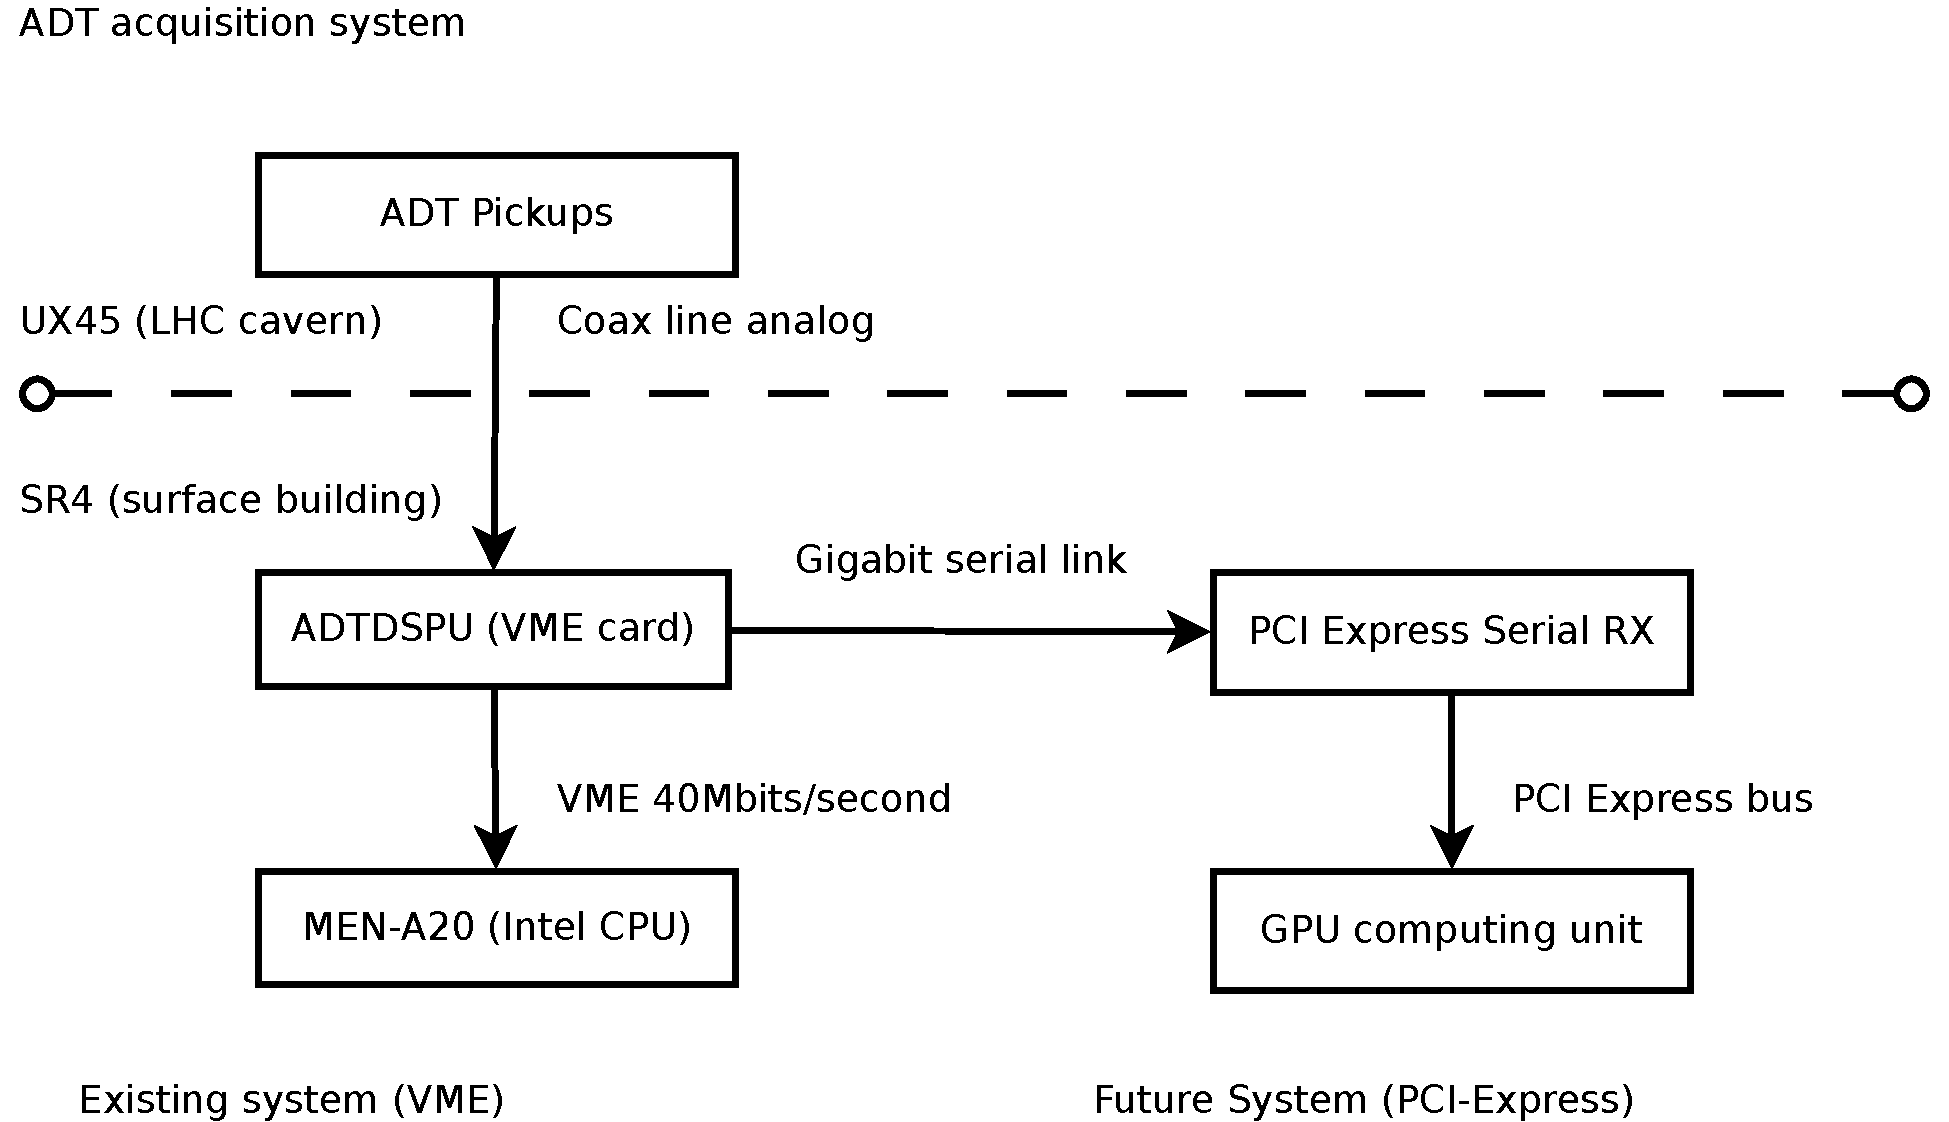
\includegraphics[scale=0.3]{acquisition.pdf}
\end{figure}

   \subsection{Software}

\section{FFT}

\section{SVD}

\section{Machine development sessions}

Using the \gls{ADT} \glspl{BPM} we acquired data in the machine during 3 independant \glspl{MD}. Most of the data taking was done in parallel to other normal LHC operation or during \gls{ADT} dedicated \gls{MD} time.

   \subsection{First session}
   
   Night session of the 11 october 2012.

   \subsection{Second session}
   
   Parasitic session of the 16 october 2012

   \subsection{Third session}

   Ramp acquisition of the 14 november 2012



\printglossaries
\bibliographystyle{plain}
\bibliography{bibliography}

\newpage
\section*{Acknowledgements}
Thanks everyone from CERN and from Heppia (TODO).

\end{document}

